%!TEX root = ../main.tex
\section{A concrete realization: the clamped--free corner under compression}
\label{sec:concrete}

The preceding analysis is deliberately abstract: it isolates the structural properties of the energy
(Assumptions~\ref{ass:reg}--\ref{ass:mild}) and of the loading (the hypotheses of \S\ref{sec:iba}) that the argument
actually uses, without committing to a domain. We now fix a concrete material and a concrete family of geometries and
ask how much of that hypothesis list can be \emph{discharged} rather than assumed. The material is the compressible
neo-Hookean energy \eqref{eq:neohooke} with the barrier penalty $f_{\log}$. The geometry is a body whose boundary
carries a clamped (Dirichlet) face meeting a traction-free (Neumann) face at a right angle, under a compressive load.

The abstract development of \S\ref{sec:asymptotics}--\S\ref{sec:iba} is already dimension-independent: it analyses the
transverse problem at the codimension-two Dirichlet--Neumann edge $\Sigma$ in $\mathbb{R}^d$. Here we instantiate it on
concrete bodies and ask how much of that hypothesis list can be \emph{discharged} rather than assumed.

\subsection{Geometry and the singular set}
\label{sub:geom}

We consider two model bodies in $\Omega\subset\mathbb{R}^d$.

\begin{itemize}
    \item \textbf{(H) Half-ball.} $\Omega = \{\,\bm{x}\in\mathbb{R}^d : |\bm{x}|<1,\ x_d>0\,\}$. The flat base
          $\Gamma_D=\{x_d=0\}\cap\partial\Omega$ is clamped; the spherical cap $\Gamma_N=\{|\bm{x}|=1\}\cap\partial\Omega$ is
          traction-free.
    \item \textbf{(C) Box.} $\Omega=(-1,1)^{d-1}\times(0,1)$. The base $\Gamma_D=\{x_d=0\}$ is clamped; the remaining faces
          are traction-free.
\end{itemize}

In both cases the load is a monotone compression transmitted through $\Gamma_N$ (a pressure or an inward normal
displacement on the cap, respectively the lateral/top faces), scaled by the pseudo-time $t\in[0,1]$ of \S\ref{sec:iba}.
We carry two bodies not because they require two analyses --- by the blow-up reduction of \S\ref{sub:blowup} they do
not, see Remark~\ref{rem:cleanmodel} --- but because they bracket the two situations one meets in practice: a globally
smooth edge (H) and a polyhedral one with vertices (C).

The \emph{singular set} $\Sigma\subset\partial\Omega$ is the locus where $\overline{\Gamma_D}$ meets
$\overline{\Gamma_N}$:
\begin{itemize}
    \item for (H), $\Sigma=\{|\bm{x}|=1,\ x_d=0\}\cong S^{d-2}$, a \emph{smooth} codimension-two submanifold; the cap is tangent
          to the vertical at the equator, so it meets the horizontal base at a right angle;
    \item for (C), $\Sigma$ is the union of the bottom edges $\{x_d=0,\ x_i=\pm1\}$, again right-angle Dirichlet--Neumann edges,
          \emph{together with} the bottom vertices, where $d$ faces meet.
\end{itemize}

Fix $\bm{x}_0\in\Sigma$ away from any vertex and split $\mathbb{R}^d=T_{\bm{x}_0}\Sigma\oplus\Pi$, with $\Pi$ the
two-plane normal to $\Sigma$. In the slice $\Pi$ the boundary reduces to a Dirichlet ray and a Neumann ray meeting at
$90^\circ$: \emph{exactly} the planar junction of \S\ref{sub:scenarioA}. We write $B_\rho$ for a tubular neighbourhood
of $\Sigma$ of radius $\rho$ and use $(r,\theta)$ for polar coordinates in $\Pi$ as before.

\begin{remark}[The two bodies are one edge analysis]
    \label{rem:cleanmodel}
    The blow-up reduction (Proposition~\ref{prop:blowup}) makes precise that (H) and (C) are \emph{not} two cases but
    one: at any non-vertex point of $\Sigma$ the transverse problem is the same planar right-angle clamped--free wedge,
    with the \emph{same} exponent $\alpha$, angular profile $\bm{\Phi}$ and reduced data, the bodies differing only
    through the scalar stress-intensity $\hat K$ (a point in the phase diagram of Remark~\ref{rem:sifparam}) and through
    edge curvature, which enters only at the subleading order $\mathcal{O}(\lambda^{g})$. The \emph{single} genuine
    distinction is topological. For (H) the singular set $\Sigma\cong S^{d-2}$ is a smooth closed manifold with no
    vertices, so the singularity is a pure edge everywhere on $\Sigma$ and the analysis holds verbatim at every point.
    For (C) the edge interiors are identical, but the bottom vertices, where $d$ faces meet, carry an additional,
    generally stronger, polyhedral-vertex singularity \cite{MazyaRossmann2010} outside the scope of the edge analysis;
    one either rounds the vertices or restricts $B_\rho$ to the edge interior. We therefore state the
    dimension-independent results once, read on (H) as the clean smooth-edge representative, and note that they hold
    verbatim on the edge interiors of (C).
\end{remark}

\subsection{The blow-up principle: reduction to the model wedge}
\label{sub:blowup}

The analysis of \S\ref{sec:asymptotics}--\S\ref{sec:iba} works on a tubular neighbourhood $B_\rho$ of $\Sigma$ cut from
a \emph{specific} body. The informal reason the two bodies of \S\ref{sub:geom} share the same corner physics is that
the singularity is localised at $\Sigma$: the leading data at the edge cannot feel the far field except through the
single amplitude $K$. We now make this precise as a blow-up (tangent-cone) reduction, which is what licenses replacing
``numerics on (H) and (C)'' by ``numerics on one universal model.''

Fix $\bm{x}_0\in\Sigma$ away from any vertex and let $W:=\Pi_W\times T_{\bm{x}_0}\Sigma$ be the \emph{tangent wedge},
with $\Pi_W=\{(r,\theta):r>0,\ 0<\theta<\tfrac\pi2\}$ the right-angle Dirichlet--Neumann quarter-plane in the normal
two-plane $\Pi$. For $\lambda\in(0,1]$ introduce the rescaling $\bm{\xi}\mapsto\bm{x}_0+\lambda\bm{\xi}$, under which
$B_{\lambda R}(\bm{x}_0)$ maps to $B_R(\bm0)\cap W$ and $\Omega_\lambda:=\lambda^{-1}(\Omega-\bm{x}_0)\to W$ as
$\lambda\to0$. Write the fundamental displacement on the loaded path as
$\bm{u}_0=K\,r^{\alpha}\bm{\Phi}(\theta)+\bm{u}_0^{\sharp}$, where by the Kondratiev expansion the remainder collects
the next exponents, $\bm{u}_0^{\sharp}=\mathcal{O}(r^{\alpha'})$ with $\alpha'>\alpha$ the second singular exponent of
the pencil, and set the \emph{spectral gap} $g:=\alpha'-\alpha>0$. Define the rescaled displacement, tangent and
operator
\begin{equation}
    \label{eq:rescale}
    \hat{\bm{u}}_\lambda(\bm{\xi}):=\lambda^{-\alpha}\big(\bm{u}_0(\bm{x}_0+\lambda\bm{\xi})-\bm{u}_0(\bm{x}_0)\big),
    \qquad
    \widehat{\mathbb{L}}_\lambda(\bm{\xi}):=\mathbb{L}\big(\bm{F}_0(\bm{x}_0+\lambda\bm{\xi})\big),
    \qquad
    \widehat{\mathcal{L}}_\lambda:=\partial_{\bm{u}}G\big(\bm{u}_0,\cdot,0\big)\big|_{\bm{x}_0+\lambda\bm{\xi}} .
\end{equation}

\begin{proposition}[Blow-up reduction to the model wedge]
    \label{prop:blowup}
    Let $\bm{x}_0\in\Sigma$ be a non-vertex point and let $\beta_\star$ be the Fredholm weight of \S\ref{sec:asymptotics}.
    Then, as $\lambda\to0$:
    \begin{enumerate}
        \item[\textup{(i)}] \emph{Kinematics.} $\hat{\bm{u}}_\lambda\to\hat{\bm{u}}_W:=K\,r^{\alpha}\bm{\Phi}(\theta)$ in
              $V^{1,2}_{\beta_\star}(B_R\cap W)$ for every $R>0$, with rate
              $\|\hat{\bm{u}}_\lambda-\hat{\bm{u}}_W\|_{V^{1,2}_{\beta_\star}(B_R\cap W)}=\mathcal{O}(\lambda^{g})$. The
              limit solves the homogeneous linear pencil on $W$ and is fixed by the wedge geometry up to the scalar $K$.
        \item[\textup{(ii)}] \emph{Operator convergence away from the tip; common intermediate pencil.} On every annulus
              $\{0<r_0\le r\le R\}\cap W$ bounded away from the vertex, the coefficients of $\widehat{\mathcal{L}}_\lambda$
              converge in $C^0$, with rate $\mathcal{O}(\lambda^{g})$, to those of the model-wedge operator
              $\mathcal{L}_W$ obtained by freezing along the self-similar field $\hat{\bm{u}}_W$. The leading singular
              exponent $\alpha$ and angular profile $\bm{\Phi}$ are \emph{intermediate-range} data: they are identical
              for $\widehat{\mathcal{L}}_\lambda$, $\mathcal{L}_W$ and the linearised-elasticity operator alike on the
              matching region $r\gg r_{\hat K}$, where the frozen field is a small perturbation of the identity and all
              three operators reduce to constant-coefficient linear elasticity, with the crossover radius
              $r_{\hat K}\to0$ as $\hat K\to0$. They are \emph{not} asserted to be vertex-pencil data of the nonlinear
              operators: at the tip the deviation of the coefficients from linear elasticity does not vanish for any
              $\hat K\neq0$, and on the tensile side the vertex pencil stabilises instead to the screened
              (vector-Laplacian) limit of Theorem~\ref{thm:A}(A), whose exponents all exceed one --- so the $r^\alpha$
              field remains the dominant asymptotics visible from any fixed scale, which is exactly what the
              universality claim uses. Thus only the dimensionless amplitude $K$ (equivalently the
              normalised stress-intensity $\hat K$ of Remark~\ref{rem:sifparam}) survives from the global problem. We
              emphasise what is \emph{not} asserted: the away-from-tip convergence does not control the operator in a
              weighted norm \emph{up to} $r=0$; at the compressive corner no screening is available (the inverse
              channel $J\to0$ drives the tangent up, and the non-compressive hypothesis behind
              Lemma~\ref{lem:Abound} fails at the tip), so the agreement of the full Lyapunov--Schmidt reduced data is
              a leading-order statement rather than a quantitative $\mathcal{O}(\lambda^{g})$ spectral-perturbation
              theorem, a uniform-to-the-tip estimate requiring the inner vertex theory left open in
              Remark~\ref{rem:core}.
        \item[\textup{(iii)}] \emph{Dimensional reduction $d\ge3\Rightarrow d=2$.} Since $\Sigma$ is smooth and the
              coefficients are constant along $T_{\bm{x}_0}\Sigma$ in the limit, the Fourier transform in the edge variable
              $\bm{s}\in T_{\bm{x}_0}\Sigma$ decomposes $\mathcal{L}_W$ into a one-parameter family
              $\{\mathcal{L}_W(\bm{\zeta})\}_{\bm{\zeta}\in\widehat{T_{\bm{x}_0}\Sigma}}$ of operators on the planar
              quarter-plane $\Pi_W$, each the transverse two-dimensional pencil of \eqref{eq:kondratiev}; the leading edge
              exponent is carried by the zero wavenumber $\bm{\zeta}=\bm0$. The model problem is therefore genuinely
              two-dimensional.
    \end{enumerate}
\end{proposition}

\begin{proof}
    Statement (i) is the leading-term extraction of the Kondratiev--Maz'ya--Rossmann expansion
    \cite{KMR2001,MazyaRossmann2010}: on the Fredholm weight $\beta_\star$ the solution admits
    $\bm{u}_0=K r^{\alpha}\bm{\Phi}+\mathcal{O}(r^{\alpha'})$, and the rescaling \eqref{eq:rescale} maps the leading term
    to the $\lambda$-independent field $K r^{\alpha}\bm{\Phi}$ exactly while shrinking the remainder by
    $\lambda^{\alpha'-\alpha}=\lambda^{g}$ in the homogeneous weighted norm. Statement (ii) follows because
    $\mathbb{L}$ is a smooth (algebraic) function of $\bm{F}_0=\bm{I}+\Grad\bm{u}_0$ and $\Grad\hat{\bm{u}}_\lambda\to
        \Grad\hat{\bm{u}}_W$ off the tip by (i); freezing along the self-similar limit defines $\mathcal{L}_W$, and the
    coefficient error inherits the $\mathcal{O}(\lambda^{g})$ rate of (i) on every annulus
    $\{r_0\le r\le R\}$ bounded away from $r=0$. The leading exponent and angular profile are read on the matching
    region: for $r\gg r_{\hat K}$ the frozen coefficients of $\widehat{\mathcal{L}}_\lambda$ and of $\mathcal{L}_W$
    alike are $\mathcal{O}((r/r_{\hat K})^{-(1-\alpha)})$-close to constant-coefficient linear elasticity at
    $\bm{x}_0$, whose Kondratiev data $(\alpha,\bm{\Phi})$ therefore govern both operators on that range,
    independently of $\lambda$; on the tensile side Theorem~\ref{thm:A}(A) guarantees in addition that the vertex
    contributes no competing exponent below one, so $(\alpha,\bm{\Phi})$ is the leading visible asymptotics. We do
    \emph{not} claim a weighted operator-norm estimate uniform up to $r=0$:
    the tip contributes through the weight, not through the body, and its quantitative control is the open inner problem
    of Remark~\ref{rem:core}; accordingly the agreement of the full reduced bifurcation data is asserted only at leading
    order. Statement (iii) is the standard edge-to-corner reduction: translation
    invariance along $T_{\bm{x}_0}\Sigma$ in the limit diagonalises $\mathcal{L}_W$ under the partial Fourier transform,
    and each fibre is the planar pencil whose smallest root is $\alpha$, attained at $\bm{\zeta}=\bm0$ (the cited edge
    calculus). \qed
\end{proof}

\begin{remark}[The one surviving global datum, and what it costs]
    \label{rem:sifparam}
    Proposition~\ref{prop:blowup} isolates exactly what does and does not localise. The exponent $\alpha$, the angular
    profile $\bm{\Phi}$, and the wedge operator $\mathcal{L}_W$ are \emph{universal}: functions of the opening
    ($90^\circ$) and the Poisson ratio alone. The only trace of the finite body is the scalar $K$, conveniently made
    dimensionless as $\hat K:=K\,\rho^{\,\alpha-1}/\mu_e$ (the normalised stress-intensity over the neighbourhood scale).
    Thus every quantity in the corner reduces to a computation on $\mathcal{L}_W$ as a function of $(\nu,\hat K)$ --- a
    two-parameter \emph{phase diagram}, not a per-body spot check. Whether a given quantity depends on $\hat K$ at all,
    or only on $(\nu)$, is decided by a homogeneity count against $\alpha$, carried out for the two open conditions in
    \S\ref{sub:attain} (condition (BC), which needs only $\nu$) and \S\ref{sub:bcount} (the cubic $b$, which retains the
    $\hat K$-dependence). This is the precise, and sharper, replacement for ``the singularity is localised to the
    corner.''
\end{remark}

\subsection{Tier 1: the material assumptions are already discharged}
\label{sub:tier1}

For the neo-Hookean energy \eqref{eq:neohooke} with $f_{\log}$, the standing assumptions of \S\ref{sec:asymptotics}
hold with explicit constants and require no information about the domain: Assumption~\ref{ass:reg} (regularity,
objectivity, and the collapse barrier $f_{\log}(J)\to\infty$), Assumption~\ref{ass:growth} (the inverse-channel bound,
with $\Theta=\Theta_{\log}$ of \eqref{eq:Thetalog}), Assumption~\ref{ass:ellip} and the sharper
Lemma~\ref{lem:SEcompress} (strong ellipticity with constant $\ge\mu_e$ throughout compression), and
Assumption~\ref{ass:mild} (logarithmic growth, $p=1$) are all established in Lemma~\ref{lem:nh},
Remark~\ref{rem:SEcaveat} and \S\ref{sub:growth}. None of these proofs uses $d=2$: the tangent formula \eqref{eq:Lnh},
the rank-one identity \eqref{eq:LHnh}, and the growth functions \eqref{eq:Thetalog} are algebraic identities in
$\mathrm{GL}^+(d)$. Thus the entire material side of the hypothesis list is closed for the concrete model, in every
dimension. What remains are the hypotheses on the \emph{solution and loading}, which is where the geometry enters.

\subsection{The edge exponent and the scenario it selects}
\label{sub:edgeexp}

By the edge-singularity calculus \cite{KMR2001,MazyaRossmann2010}, the leading singular exponents of the linearised
elasticity operator along the smooth edge $\Sigma$ coincide with those of the transverse two-dimensional pencil in
$\Pi$, modulated smoothly along $\Sigma$. That transverse pencil is the planar right-angle Dirichlet--Neumann corner of
\eqref{eq:kondratiev}; its leading exponent $\alpha\in(0,1)$ is the smallest root of the corresponding clamped--free
Williams secular equation and depends only on the Poisson ratio. Consequently the kinematic blow-up \eqref{eq:Fblowup},
$\bm{F}=\bm{I}+\mathcal{O}(r^{\alpha-1})$, holds with a \emph{computable} exponent, and by Theorem~\ref{thm:A} the
nonlinear tangent inherits exactly this $\alpha$ in the benign regime on the intermediate annulus outside the
nonlinear crossover scale (and outside the dilation core of Lemma~\ref{lem:Aellip}), while at the vertex itself the
tensile tangent stabilises to the screened Laplacian limit, which contributes no competing exponent below one.

Which scenario of \S\ref{sec:asymptotics} is realized is governed by the sign of the dominant eigenvalue of
$\Grad\bm{u}$ at the edge, equivalently by the sign of the stress-intensity factor $K$ in \eqref{eq:kondratiev}. This
is a global quantity, set by the far field, and is not determined by the local pencil alone. The compressive load we
impose selects $K<0$: the material is pushed into the corner, the dominant eigenvalue of $\Grad\bm{u}$ is negative, and
Scenario~B (\S\ref{sub:scenarioB}) is the relevant branch. The quantitative form of ``compressive enough'' is the
hypothesis (SC) below; it simultaneously selects Scenario~B and drives the structural instability of
\S\ref{sub:concrete-tc}. The complementary tensile load ($K>0$) selects Scenario~A, where (NC) holds and
Theorem~\ref{thm:A} applies; for the present geometry under compression that case does not arise near the edge.

\subsection{Existence of the critical load via a localized surface instability}
\label{sub:concrete-tc}

The one genuinely non-elementary ingredient of \S\ref{sec:iba} was hypothesis (ii) of Lemma~\ref{lem:tc}: the existence
of a structurally destabilising field, $Q_{t_*}(\bm{v}_*)<0$, which we there declined to establish and flagged as the
corner counterpart of the Biot/creasing instability. For the concrete clamped--free geometry we now \emph{prove} it, by
reduction to the surface instability of the compressed half-space.

The free face $\Gamma_N$ under compression is, locally, a traction-free surface compressed parallel to itself --- the
exact configuration of Biot's classical analysis \cite{Biot1963}. A homogeneously compressed neo-Hookean half-space
loses stability to a surface mode once the surface-parallel stretch falls below a threshold $\lambda_\star\in(0,1)$
(for the incompressible model $\lambda_\star\approx0.544$; for the compressible energy \eqref{eq:neohooke} the
threshold is the corresponding root of the surface secular equation, still in $(0,1)$ \cite{Hong2009}). We package the
loading requirement as a single hypothesis.

\begin{assumption}[Surface compression reaches threshold, (SC)]
    \label{ass:sc}
    There exist $t_*\in(0,1]$ and an interior point $P\in\Gamma_N\cap B_\rho$, at positive distance from both $\Sigma$
    and $\overline{\Gamma_D}$, such that the fundamental state compresses the free face below the half-space threshold
    there: the surface-parallel principal stretch of $\bm{F}_0(t_*)$ at $P$ satisfies
    $\lambda_\parallel\big(\bm{F}_0(t_*);P\big)<\lambda_\star$.
\end{assumption}

\noindent (SC) is an input on the \emph{loading}, in the same spirit as the monotonicity condition (M) of
Lemma~\ref{lem:transversal}: it says only that the prescribed compression is strong enough that the free surface dips
below its own buckling threshold somewhere near the edge. Since $t$ merely normalises the load amplitude, (SC) can
always be met by loading hard enough, provided the material does not fail elsewhere first.

\begin{lemma}[Localized surface instability $\Rightarrow$ structural instability]
    \label{lem:biot}
    Under Assumption~\ref{ass:sc}, hypothesis (ii) of Lemma~\ref{lem:tc} holds: there is $\bm{v}_*\in V$, supported in
    $B_\rho$ and vanishing on $\Gamma_D$, with
    \begin{equation}
        \label{eq:Qneg}
        Q_{t_*}(\bm{v}_*) = \int_{B_\rho}\Grad\bm{v}_* : \mathbb{L}\big(\bm{F}_0(t_*)\big) : \Grad\bm{v}_*\,dV < 0 .
    \end{equation}
    Consequently, with $\mu_1(0)>0$ from Lemma~\ref{lem:tc}(i), there is a first critical load $t_c\in(0,t_*]$ with
    $\mu_1(t_c)=0$.
\end{lemma}

\begin{proof}
    Work in coordinates centred at $P$: let $n\ge0$ be the depth into the body along the inward normal to $\Gamma_N$ and
    $\bm{s}\in\mathbb{R}^{d-1}$ the surface-tangent coordinates, so that near $P$ the body is the half-space $\{n>0\}$ and
    $\bm{F}_0(t_*)$ is $C^1$ with value $\bm{F}_P:=\bm{F}_0(t_*;P)$ whose surface-parallel stretch is
    $\lambda_\parallel<\lambda_\star$.

    \emph{Step 1: the homogeneous unstable mode.} Freeze the coefficients at $\bm{F}_P$ and consider the constant-tensor
    form $Q_0(\bm{v})=\int_{\{n>0\}}\Grad\bm{v}:\mathbb{L}(\bm{F}_P):\Grad\bm{v}\,dV$ on the half-space, with $\bm{v}$
    traction-free at $n=0$. Because $\lambda_\parallel<\lambda_\star$, the half-space is past its surface-instability
    threshold \cite{Biot1963,Hong2009}: for each surface wavevector $\bm{k}\in\mathbb{R}^{d-1}$, $k:=|\bm{k}|$, there is a
    surface mode
    \begin{equation}
        \label{eq:biotmode}
        \bm{v}_{\bm{k}}(\bm{s},n) = \mathrm{Re}\,\big[\,\hat{\bm{v}}(kn)\,e^{\mathrm{i}\bm{k}\cdot\bm{s}}\,\big],
        \qquad |\hat{\bm{v}}(\zeta)|\le C e^{-\beta\zeta}\ (\beta>0),
    \end{equation}
    decaying exponentially into the body on the depth scale $1/k$. Since $\mathbb{L}(\bm{F}_P)$ is constant, the rescaling
    $(\bm{s},n)\mapsto k^{-1}(\bm{s},n)$ shows that over a surface window $W$ of area $|W|$,
    \begin{equation}
        \label{eq:biotscale}
        \int_{\{n>0\}} \mathbf{1}_W\,\Grad\bm{v}_{\bm{k}}:\mathbb{L}(\bm{F}_P):\Grad\bm{v}_{\bm{k}}\,dV
        = q(\lambda_\parallel)\,k\,|W|\,(1+o(1)), \qquad q(\lambda_\parallel)<0,
    \end{equation}
    where $q$ is the Biot secular form, strictly negative past threshold. Likewise
    $\int_{\{n>0\}}\mathbf{1}_W\,|\Grad\bm{v}_{\bm{k}}|^2 \sim k\,|W|$ and
    $\int_{\{n>0\}}\mathbf{1}_W\,|\bm{v}_{\bm{k}}|^2 \sim k^{-1}|W|$, the latter two by the same scaling.

    \emph{Step 2: cut-off.} Let $\chi$ be smooth, $\chi\equiv1$ on $B(P,\delta/2)$, $\mathrm{supp}\,\chi\subset
        B(P,\delta)$, $|\Grad\chi|\le C/\delta$, with $\delta$ small enough that $B(P,\delta)\cap\overline\Omega$ avoids
    both $\Sigma$ and $\overline{\Gamma_D}$ and lies in $B_\rho$ (possible since $P$ is at positive distance from both).
    Set $\bm{v}_*:=\chi\,\bm{v}_{\bm{k}}$. Then $\bm{v}_*\in V$ and vanishes on $\Gamma_D$ (its support avoids
    $\overline{\Gamma_D}$); it is unconstrained on the free face, as required.

    \emph{Step 3: error control.} Write $\Grad\bm{v}_*=\chi\Grad\bm{v}_{\bm{k}}+(\Grad\chi)\otimes\bm{v}_{\bm{k}}$ and
    expand \eqref{eq:Qneg}. The effective window is $W\sim B(P,\delta)\cap\Gamma_N$, of area $|W|\sim\delta^{d-1}$, and the
    decay confines the mass to depth $1/k$. Three errors arise.
    \begin{enumerate}
        \item[(a)] \emph{Coefficient variation:} replacing $\mathbb{L}(\bm{F}_0(\bm{x}))$ by $\mathbb{L}(\bm{F}_P)$ costs
              $\le \sup_{B(P,\delta)}\|\mathbb{L}(\bm{F}_0)-\mathbb{L}(\bm{F}_P)\|\int\chi^2|\Grad\bm{v}_{\bm{k}}|^2
                  \le C\delta\cdot k\delta^{d-1}=Ck\delta^{d}$ (by $C^1$ regularity of $\bm{F}_0$ at $P$).
        \item[(b)] \emph{Gradient commutator:} the cross term and $|\Grad\chi|^2|\bm{v}_{\bm{k}}|^2$ term are bounded by
              $C\big(\delta^{-1}\!\!\int_W |\bm{v}_{\bm{k}}||\Grad\bm{v}_{\bm{k}}| + \delta^{-2}\!\!\int_W|\bm{v}_{\bm{k}}|^2\big)
                  \le C\big(\delta^{d-2} + \delta^{d-3}k^{-1}\big)$.
        \item[(c)] \emph{Window vs.\ cut-off:} replacing $\mathbf{1}_W$ by $\chi^2$ in \eqref{eq:biotscale} changes the
              leading constant by $1+o(1)$ only.
    \end{enumerate}
    The leading term is $q(\lambda_\parallel)\,k\,\delta^{d-1}<0$. The errors (a)--(b), relative to it, are
    $\mathcal{O}(\delta)$, $\mathcal{O}((k\delta)^{-1})$ and $\mathcal{O}((k\delta)^{-2})$. Choosing $\delta=k^{-1/2}$
    sends $\delta\to0$ and $k\delta=k^{1/2}\to\infty$, so all relative errors vanish as $k\to\infty$. Hence for $k$ large
    enough,
    \[
        Q_{t_*}(\bm{v}_*) = q(\lambda_\parallel)\,k\,\delta^{d-1}\,(1+o(1)) < 0,
    \]
    which is \eqref{eq:Qneg}. The final statement is Lemma~\ref{lem:tc} with hypothesis (ii) now supplied. \qed
\end{proof}

\begin{remark}[What this closes]
    Lemma~\ref{lem:biot} converts the existence of the critical load $t_c$ --- previously conditional on the unproved
    hypothesis (ii) --- into a \emph{theorem} for the concrete clamped--free geometry, contingent only on the loading
    hypothesis (SC). What the construction delivers, and what it does not, should be stated precisely. It exhibits a
    single admissible field $\bm{v}_*$ with $Q_{t_*}(\bm{v}_*)<0$, which by Lemma~\ref{lem:tc} is all that is needed to
    force a crossing $\mu_1(t_c)=0$ at some $t_c\in(0,t_*]$. The destabilising mechanism is the half-space surface
    (creasing) instability, seated at an interior free-face point $P$ of the edge neighbourhood $B_\rho$ and confined to
    it by the cut-off \eqref{eq:biotmode}--\eqref{eq:biotscale}; the witness $\bm{v}_*$ is supported away from the tip
    $r=0$ (indeed (SC) places $P$ at positive distance from $\Sigma$), so the lemma certifies a surface instability
    \emph{within $B_\rho$}, not a mode pinned at the corner vertex. This is the precise sense in which the corner
    bifurcation is ``the corner analogue of creasing'': the same free-face mechanism, activated near --- not at --- the
    edge. The location and shape of the genuine \emph{critical} mode $\bm{\phi}$ at $t_c$ is a separate question,
    settled by the attainment analysis of \S\ref{sub:attain} (which gives $\bm{\phi}\in V$ supported in $B_\rho$), and
    the role of the edge proper enters quantitatively only through the graded pre-stress of Remark~\ref{rem:twoscales}.
\end{remark}

\begin{remark}[On the threshold $\lambda_\star$: compressible vs.\ incompressible]
    \label{rem:threshold}
    The proof uses only the \emph{existence} of a surface-instability threshold $\lambda_\star\in(0,1)$, not its value.
    The familiar number $\lambda_\star\approx0.544$ is Biot's result for the \emph{incompressible} neo-Hookean half-space
    \cite{Biot1963}; the present material \eqref{eq:neohooke} is compressible, and its threshold is the corresponding root
    of the compressible surface secular equation, which depends on the ratio $\lambda_e/\mu_e$ (equivalently the Poisson
    ratio) and tends to $0.544$ in the incompressible limit $\lambda_e/\mu_e\to\infty$ \cite{Hong2009}. This is the same
    instability with a material-dependent threshold, not a discrepancy: Lemma~\ref{lem:biot} \emph{reduces} the corner
    instability to the half-space one and thereby agrees with the creasing literature rather than competing with it.
    Accordingly we keep $\lambda_\star$ symbolic throughout.
\end{remark}

\subsection{Symmetry: simplicity of the mode and the vanishing quadratic}
\label{sub:symmetry}

Both model bodies of \S\ref{sub:geom} possess reflection symmetries that the fundamental compressive state inherits:
(H) is invariant under every orthogonal map fixing the $x_d$-axis, and (C) under each coordinate reflection
$x_i\mapsto-x_i$ ($i<d$). Let $R$ be such a reflection and $\mathcal{R}$ its action on displacement fields. Because
$\bm{F}_0(t)$ and hence $\mathbb{L}(\bm{F}_0(t))$ are $R$-invariant, the second-variation operator $\mathcal{L}(t)$
commutes with $\mathcal{R}$, so its eigenspaces split into the symmetric ($\mathcal{R}=+1$) and antisymmetric
($\mathcal{R}=-1$) sectors. This yields, for the concrete geometry, two of the ingredients that \S\ref{sec:iba} had to
posit:

\begin{itemize}
    \item \emph{Simplicity (part of Assumption~\ref{ass:bif}).} The symmetry splitting reduces simplicity to two
          residual statements --- that the crossing eigenvalue is the ground state of its sector, and that no
          accidental degeneracy across sectors occurs at $t_c$. Calling these \emph{generic} requires a parameter to
          be perturbed, and for the fixed body none is; the honest formulation uses the family the paper already
          works on. For a real self-adjoint family, eigenvalue coincidence is a codimension-\emph{two} event
          (von Neumann--Wigner), so within the two-parameter wedge family $(\nu,\hat K)$ the loads at which the
          one-parameter path $t\mapsto\mathcal{L}(t)$ meets a degeneracy are avoided at the crossing for almost every
          $(\nu,\hat K)$; both residual statements then hold off a null set of the phase diagram, though not
          pointwise for a given body. At tested points they are moreover \emph{checked}, not assumed: the sector gap
          computed in \S\ref{sub:numb} is exactly this quantity --- with the caveat, recorded there, that its
          behaviour under refinement is not yet settled. With that framing, simplicity need not be assumed as an
          independent spectral postulate, and only the \emph{attainment} clause (the borderline-elliptic point of
          Remark~\ref{rem:framework}) requires the separate analysis of \S\ref{sub:attain}.
    \item \emph{Vanishing quadratic coefficient (part of Assumption~\ref{ass:subcrit}).} The reduced potential of
          Proposition~\ref{prop:LS} inherits the $\mathcal{R}$-symmetry of the perfect state. If $\bm{\phi}$ lies in the
          antisymmetric sector, $w\mapsto-w$ is a symmetry of the reduced equation and the quadratic coefficient
          vanishes. For the neo-Hookean model this is made fully explicit in Lemma~\ref{lem:volcoeff}: $c_2$ is odd in
          the first-order volume change $D_1$, which $R$ flips, so $c_2=0$ exactly. The relevant reflection $R$ is the
          lateral, \emph{face-preserving} symmetry of the model bodies of \S\ref{sub:geom}, \emph{not} the corner
          bisector (which would interchange $\Gamma_D$ and $\Gamma_N$ and is no symmetry of the mixed problem).
\end{itemize}

\begin{lemma}[Neo-Hookean reduced coefficients are volumetric; the quadratic vanishes]
    \label{lem:volcoeff}
    For the neo-Hookean energy \eqref{eq:neohooke} the deviatoric term $\tfrac{\mu_e}{2}(\tr\bm F^T\bm F-d)$ is quadratic
    in $\bm F$, so its third and higher Fr\'echet derivatives vanish; hence \emph{every} reduced bifurcation coefficient
    of order $\ge3$ is purely volumetric, determined by $f$ alone. Writing
    $J(w)=\det(\bm F_0+w\Grad\bm\phi)=\sum_k D_k\,w^k$ with $D_k$ the mixed discriminants of Lemma~\ref{lem:relief}
    ($D_1=\operatorname{cof}\bm F_0:\Grad\bm\phi$, $D_2=d_\phi$, $D_{k}=0$ for $k>d$) and $f^{(k)}=f^{(k)}(J_0)$, the
    single-mode coefficients are
    \begin{align}
        \label{eq:c2vol}
        c_2              & = \tfrac12\!\int_{B_\rho}\!\big[f''' D_1^3+6 f'' D_1 D_2+6 f' D_3\big]\,dV, \\
        \label{eq:bvol}
        b_{\mathrm{dir}} & = \tfrac16\!\int_{B_\rho}\!\big[f'''' D_1^4+12 f''' D_1^2 D_2+12 f'' D_2^2
            +24 f'' D_1 D_3+24 f' D_4\big]\,dV.
    \end{align}
    Two consequences hold for the concrete geometry, whose fundamental state is $R$-symmetric.
    \begin{enumerate}
        \item[\textup{(i)}] \emph{The quadratic vanishes, exactly and without correction.} As a \emph{third}-order
              quantity $c_2$ receives no orthogonal-mode (Lyapunov--Schmidt) feedback --- that correction first enters
              at fourth order --- so \eqref{eq:c2vol} is the full $c_2$. The key parity fact is that each mixed
              discriminant $D_k=\tfrac1{k!}\partial_w^k\det(\bm F_0+w\Grad\bm\phi)|_0$ is exactly the degree-$k$ part of
              the determinant in $\Grad\bm\phi$, hence carries $k$ factors of $\Grad\bm\phi$ and one factor of an
              $R$-even cofactor of $\bm F_0$ per term. For an $R$-antisymmetric mode $\Grad\bm\phi$ reverses sign under
              the reflection (composed with the change of variables $\bm x\mapsto R\bm x$ on the $R$-symmetric domain
              $B_\rho$), so $D_k$ acquires the parity $(-1)^k$: $D_1$ and $D_3$ are $R$-odd, $D_2$ is $R$-even, while
              $f^{(k)}(J_0)$ is $R$-even (the base state is $R$-invariant). Each term of \eqref{eq:c2vol} thus carries an
              \emph{odd} total number of $\Grad\bm\phi$ factors --- $D_1^3$ (three), $D_1D_2$ (three), and $D_3$ (three)
              --- and is therefore $R$-odd; the integrand is odd over the $R$-symmetric $B_\rho$ and $c_2=0$. (In $d=2$
              the term $6f'D_3$ is moreover identically zero, since $D_k=0$ for $k>d$; the parity argument is what
              disposes of it in $d\ge3$.) This \emph{proves} the vanishing-quadratic clause of
              Assumption~\ref{ass:subcrit}.
        \item[\textup{(ii)}] \emph{The frozen cubic and quintic are sign-definite, and adverse to subcriticality.} With
              $D_1$ asymptotically small (Assumption~\ref{ass:rot}), the leading frozen
              parts are $b_{\mathrm{dir}}=2\int_{B_\rho} f''(J_0)\,d_\phi^2\,dV$ and
              $d_{\mathrm{dir}}=\int_{B_\rho} f'''(J_0)\,d_\phi^3\,dV$. For the logarithmic penalty
              $f''_{\log}(J_0)=(\mu_e+2\lambda_e-2\lambda_e\log J_0)/J_0^2>0$ and
              $f'''_{\log}(J_0)=(4\lambda_e\log J_0-6\lambda_e-2\mu_e)/J_0^3<0$ throughout compression $J_0<1$. The cubic
              part carries $d_\phi^2\ge0$, so $b_{\mathrm{dir}}>0$ follows from $f''_{\log}>0$ \emph{alone}, with no sign
              hypothesis on $d_\phi$ (this is the only frozen sign the argument needs). The quintic part carries the
              sign-indefinite $d_\phi^3$; on the relief-oriented region $d_\phi>0$ (\eqref{eq:dphisign} below) and
              $f'''_{\log}<0$ give $d_{\mathrm{dir}}<0$ there --- the \emph{opposite} of the subcritical pattern $b<0<d$, so
              the frozen quintic too is adverse where the relief acts, and subcriticality is decided by the feedback, not
              by either frozen term.
    \end{enumerate}
\end{lemma}
\begin{proof}
    Expand $\Psi(\bm F_0+w\Grad\bm\phi)=\tfrac{\mu_e}2(\tr\bm F^T\bm F-d)+f(J(w))$ in $w$. The deviatoric part is a
    polynomial of degree two in $w$, so it contributes only to the coefficients of $w^0,w^1,w^2$; all coefficients of
    order $\ge3$ come from $f(J(w))$, whose $w$-derivatives are given by Fa\`a di Bruno's formula in the
    $J$-derivatives $f^{(k)}$ and the discriminants $D_k=\tfrac1{k!}\partial_w^k\det(\bm F_0+w\Grad\bm\phi)|_0$. Reading
    off the third and fourth derivatives gives \eqref{eq:c2vol}--\eqref{eq:bvol}; statements (i)--(ii) are then as
    stated, using $f''_{\log}>0$, $f'''_{\log}<0$ on $J_0<1$. \qed
\end{proof}

What symmetry fixes is thus the quadratic coefficient; what it does \emph{not} fix is the sign of the cubic $b$ and
quintic $d$. Indeed the explicit single-mode parts \eqref{eq:bvol} point \emph{against} subcriticality
($b_{\mathrm{dir}}>0$, $d_{\mathrm{dir}}<0$ by Lemma~\ref{lem:volcoeff}(ii)), so the subcritical pattern $b<0<d$ rests
entirely on the geometry-dependent orthogonal-mode feedback --- the irreducible core, which we settle numerically
rather than by analogy (Remark~\ref{rem:bsign}). Proposition~\ref{prop:bcount} below explains, by a homogeneity count
against the edge exponent $\alpha$, \emph{why} this feedback cannot be reduced to a universal corner number.

\subsection{The homogeneity count for the cubic}
\label{sub:bcount}

The blow-up reduction of \S\ref{sub:blowup} promised a dichotomy: a corner quantity localises to a universal
model-wedge number only when its defining integral is dominated by the tip. We now carry out the count for the cubic
coefficient and find that, for the right-angle clamped--free pencil, it sits on the \emph{non}-localising side ---
which is exactly why the sign of $b$ is a genuine, $\hat K$-dependent computation rather than an inheritance from flat
creasing.

Near the edge the critical mode $\bm{\phi}\in V$ inherits the admissible singular behaviour of the pencil,
$\Grad\bm{\phi}=\mathcal{O}(r^{\alpha-1})$ (the least-singular $H^1$ exponent of \eqref{eq:kondratiev}), so the second
discriminant scales as $d_\phi=\det\Grad\bm{\phi}=\mathcal{O}(r^{2(\alpha-1)})$ in $d=2$.

\begin{proposition}[Homogeneity count: the cubic does not localise to the bare wedge]
    \label{prop:bcount}
    In $d=2$ the single-mode integrand of $b_{\mathrm{dir}}=2\!\int_{B_\rho}f''(J_0)\,d_\phi^2\,dV$ scales as
    $d_\phi^2=\mathcal{O}(r^{4(\alpha-1)})$, so
    \begin{equation}
        \label{eq:bcount}
        \int_{B_\rho} d_\phi^2\,dV \ \sim\ \int_0 r^{4(\alpha-1)}\,r\,dr \ =\ \int_0 r^{\,4\alpha-3}\,dr,
    \end{equation}
    which converges at the tip $r=0$ iff $4\alpha-3>-1$, i.e.\ iff $\alpha>\tfrac12$.
    \begin{enumerate}
        \item[\textup{(i)}] \emph{The clamped--free pencil lies above the threshold.} The smallest root of the
              right-angle clamped--free Williams secular equation (plane strain, $\kappa=3-4\nu$) is
              $\alpha=\alpha(\nu)\in(0.60,0.87)$ for $\nu\in(0,\tfrac12)$ --- e.g.\ $\alpha(0.3)\approx0.711$,
              $\alpha(0.45)\approx0.622$, $\alpha(0.499)\approx0.595$ --- so $\alpha>\tfrac12$ throughout the physical
              range (Figure~\ref{fig:williams}).
        \item[\textup{(ii)}] \emph{Consequence: tip-convergent but not tip-dominated.} For $\alpha>\tfrac12$ the integral
              \eqref{eq:bcount} converges \emph{without} barrier regularisation, but its mass is spread over the annulus
              rather than concentrated at the tip; the cut-off radius $\rho$ and the matching to the far field leave an
              $\mathcal{O}(1)$ residue. By Proposition~\ref{prop:blowup} this residue is carried by the normalised
              stress-intensity $\hat K$. Hence $b$ does \emph{not} collapse to a bare-wedge number: it is a functional
              $b=b(\nu,\hat K)$ on the graded-substrate creasing model (a half-space crease seated in the linear
              pre-stress gradient of the edge field), and the subcritical sign $b<0$ is the sign of $b(\nu,\hat K)$ over
              the physical $(\nu,\hat K)$ rectangle --- a two-parameter phase diagram, not a single number.
        \item[\textup{(iii)}] \emph{The complementary regime.} Were $\alpha<\tfrac12$ (e.g.\ at sharper or
              differently-loaded openings), \eqref{eq:bcount} would diverge at the tip, the barrier/collapse-locus
              regularisation of \S\ref{sub:reliefd} would render it finite, and $b$ \emph{would} be set by an
              arbitrarily small tip neighbourhood --- a genuinely localised, $\hat K$-free wedge functional. The present
              geometry is firmly in case (ii).
    \end{enumerate}
\end{proposition}

\begin{figure}[t]
    \centering
    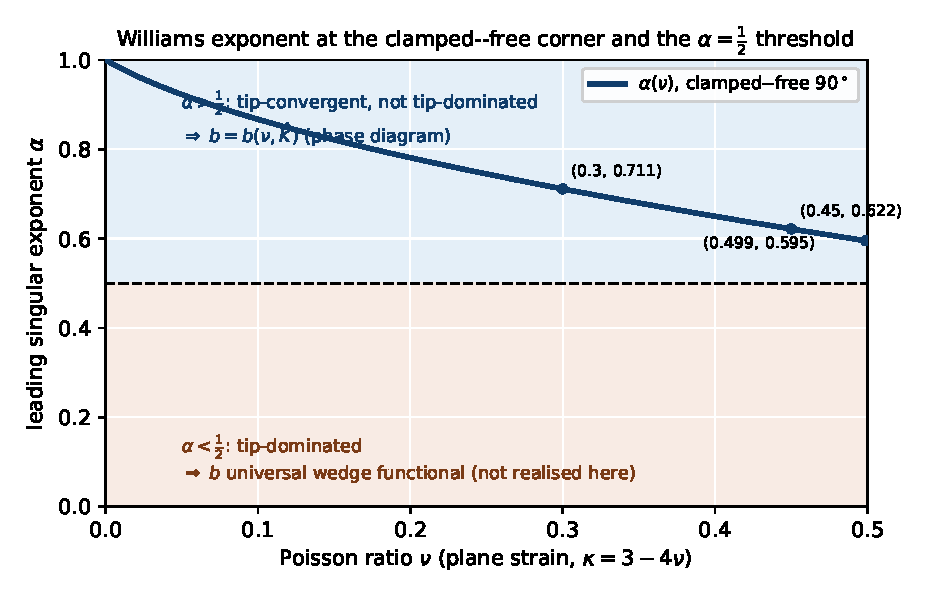
\includegraphics[width=0.72\textwidth]{figures/williams_exponent.pdf}
    \caption{Leading Williams singular exponent $\alpha(\nu)$ for the right-angle clamped--free (Dirichlet--Neumann)
        wedge (plane strain, $\kappa=3-4\nu$), the smallest root in $(0,1)$ of the $4\times4$ secular determinant of
        Proposition~\ref{prop:bcount}. Across the entire physical range the curve lies in the regime
        $\alpha>\tfrac12$ (upper band), where the cubic integral \eqref{eq:bcount} is tip-convergent but not
        tip-dominated, so the reduced coefficient retains its dependence on the normalised stress-intensity,
        $b=b(\nu,\hat K)$. The lower band $\alpha<\tfrac12$ (tip-dominated, $b$ a universal wedge functional) is not
        reached by this geometry. The exponent rises to $\alpha\to1$ as $\nu\to0$, i.e.\ the singularity \emph{weakens}
        for small Poisson ratio and the stress concentration disappears in the limit ($\bm{F}$ bounded for
        $\alpha\ge1$); this is expected, the corner stress singularity being driven by the volumetric coupling that
        vanishes as $\nu\to0$. Reproduced by \texttt{williams\_clampedfree.py} / \texttt{plot\_williams\_exponent.py}.}
    \label{fig:williams}
\end{figure}

\begin{proof}
    The scaling \eqref{eq:bcount} is immediate from $d_\phi=\det\Grad\bm{\phi}=\mathcal{O}(r^{2(\alpha-1)})$ and the
    area element $r\,dr\,d\theta$; convergence at $r=0$ is the elementary condition $4\alpha-3>-1$. The factor
    $f''(J_0)$ is bounded away from the collapse locus and only strengthens convergence under compression
    ($f''_{\log}>0$), so it does not change the count. The exponents in (i) are the smallest real roots in $(0,1)$ of
    the $4\times4$ boundary-condition determinant for the clamped ($u_r=u_\theta=0$ at $\theta=0$) and traction-free
    ($\sigma_{\theta\theta}=\sigma_{r\theta}=0$ at $\theta=\tfrac\pi2$) Kolosov--Muskhelishvili eigensolutions
    $\varphi=Cz^{\alpha}$, $\psi=Ez^{\alpha}$; the value $\alpha(0.3)\approx0.711$ reproduces the classical
    $90^\circ$ fixed--free corner. Statements (ii)--(iii) are the localisation/non-localisation alternative of the
    blow-up dichotomy (Remark~\ref{rem:sifparam}) applied to the convergent, respectively divergent, case of
    \eqref{eq:bcount}. \qed
\end{proof}

\begin{remark}[Two scales, and why flat creasing does not hand over the sign]
    \label{rem:twoscales}
    Case (ii) has a transparent mechanical reading. The buckling mode of Lemma~\ref{lem:biot} is a crease localised at
    an interior free-face point $P$ on the wavelength scale $1/k$, while the edge field varies on the scale $r_P$ of the
    distance from $P$ to $\Sigma$. If $1/k\ll r_P$ the crease sees a locally \emph{homogeneous} pre-stress and inherits
    the flat-surface sign $b<0$ for free; that limit is precisely the one $\alpha<\tfrac12$ would enforce, and it is
    \emph{not} the present case. For $\alpha>\tfrac12$ the surviving contribution lives at $1/k\sim r_P$, where the crease
    sits in the \emph{graded} pre-stress of the corner; the substrate gradient enters through $\hat K$ and the flat
    result no longer dictates the sign. This is the analytic origin of the ``$\mathcal{O}(1)$ geometry competition'' that
    makes $b$ the one irreducibly numerical coefficient.
\end{remark}

\begin{remark}[The flat reduction is degenerate; the corner is what makes $b$ exist]
    \label{rem:flatdegenerate}
    The phrase ``inherits the flat sign $b<0$'' in Remark~\ref{rem:twoscales} must be read with care, because the flat
    single-mode reduction is in fact \emph{singular}. The Biot surface-instability threshold of the homogeneous
    half-space is \emph{scale-free}: the secular condition is independent of the surface wavenumber $k$, so at
    $\lambda_\parallel=\lambda_\star$ \emph{every} harmonic is simultaneously neutral. The Lyapunov--Schmidt reduction of
    a single mode of wavenumber $k$ then feeds, at second order, a response at wavenumber $2k$ --- which is itself a
    neutral mode of the same operator. The second-harmonic problem is therefore \emph{resonant}, the orthogonal-mode
    field $\bm\psi$ does not exist as a bounded correction, and the single-mode cubic coefficient $b$ is undefined for the
    flat surface. (Numerically, the smallest singular value of the incremental operator at $\lambda_\star$ is at machine
    level for $k=1,2,3,4$ alike.) This is the precise analytic reason that flat creasing is a \emph{localised},
    finite-amplitude instability rather than a sinusoidal supercritical/subcritical bifurcation
    \cite{Hong2009}: there is no single-mode normal form to carry a sign.

    The corner removes exactly this degeneracy. The pre-stress is graded along the free face on the scale $r_P$
    (Remark~\ref{rem:twoscales}), which breaks the translational/scale invariance, couples the wavenumbers, and selects a
    \emph{discrete} critical mode --- the attainment of Lemma~\ref{lem:attain} under (BC). With the spectrum discrete and
    simple, the second-harmonic operator is no longer resonant, $\bm\psi$ exists, and $b=b(\nu,\hat K)$ is a well-defined
    number. Thus the corner is not merely the setting in which $b$ happens to be computed: it is what makes the reduced
    cubic \emph{exist} at all. This sharpens Proposition~\ref{prop:bcount} --- $b$ cannot be a bare-wedge, $\hat
        K$-independent constant, because the $\hat K\to0$ (flat) limit is not a regular point of the reduction but the
    degenerate one.
\end{remark}

The degeneracy just described is not only an obstruction; combined with the feedback-sign
Lemma~\ref{lem:fbsign}, it is a \emph{mechanism}. Near the flat limit the second harmonic is nearly neutral, so the
denominator of the certification criterion \eqref{eq:certcrit} is nearly zero --- and the feedback, which is exactly
the supremum \eqref{eq:fbvar}, is correspondingly large. This can be turned into a theorem for the small-$\hat K$
regime.

\begin{proposition}[Certified subcriticality at the edge of the flat degeneracy]
    \label{prop:certdeg}
    Let $\{(\bm{\phi}_{\hat K},\mathcal{L}_{c,\hat K})\}_{\hat K>0}$ be the family of critical states of the graded
    reduction (Proposition~\ref{prop:bcount}(ii)), and for each $\hat K$ let $\bm{v}_{\hat K}\in V^\perp$ be an
    admissible comparison field --- the natural candidate is the doubled-wavenumber surface harmonic, which by
    Remark~\ref{rem:flatdegenerate} goes neutral in the flat limit. With $E_3$ and $b_{\mathrm{dir}}$ as in
    Lemma~\ref{lem:fbsign}, set the (scaling-invariant in both $\bm\phi$ and $\bm v$) certification ratio
    \begin{equation}
        \label{eq:gammadef}
        \Gamma(\hat K) := \frac{E_3[\bm{\phi}_{\hat K},\bm{\phi}_{\hat K},\bm{v}_{\hat K}]^2}
        {2\,b_{\mathrm{dir}}(\hat K)\,\langle\bm{v}_{\hat K},\mathcal{L}_{c,\hat K}\bm{v}_{\hat K}\rangle}\ ,
    \end{equation}
    so that, by Corollary~\ref{cor:cert}, $b\le b_{\mathrm{dir}}\,(1-\Gamma)$ and $b(\nu,\hat K)<0$ whenever
    $\Gamma(\hat K)>1$. Suppose that, as $\hat K\to0^+$,
    \begin{enumerate}
        \item[\textup{(a)}] the comparison field goes neutral,
              $\langle\bm{v},\mathcal{L}_c\bm{v}\rangle/\|\bm{v}\|_V^2\to0$ (the flat resonance of
              Remark~\ref{rem:flatdegenerate}); and
        \item[\textup{(b)}] the second-harmonic coupling does not degenerate along with it:
              $E_3[\bm{\phi},\bm{\phi},\bm{v}]^2/\big(b_{\mathrm{dir}}\,\|\bm{v}\|_V^2\big)\ \ge\ c_0>0$ uniformly in
              $\hat K$.
    \end{enumerate}
    Then $\Gamma(\hat K)\to\infty$; in particular there is $\hat K_0>0$ such that $b(\nu,\hat K)<0$ for all
    $\hat K\in(0,\hat K_0)$, with diverging margin, $b_\psi/b_{\mathrm{dir}}\le-\Gamma\to-\infty$.
\end{proposition}

\begin{proof}
    Immediate from Corollary~\ref{cor:cert}:
    $\Gamma=\big[E_3^2/(b_{\mathrm{dir}}\|\bm{v}\|_V^2)\big]\cdot
        \big[2\langle\bm{v},\mathcal{L}_c\bm{v}\rangle/\|\bm{v}\|_V^2\big]^{-1}
        \ge \tfrac12\,c_0\,\big[\langle\bm{v},\mathcal{L}_c\bm{v}\rangle/\|\bm{v}\|_V^2\big]^{-1}\to\infty$
    by (a)--(b), and $b\le b_{\mathrm{dir}}(1-\Gamma)$ with $b_{\mathrm{dir}}>0$. \qed
\end{proof}

\begin{remark}[Reading, and the computational route it recommends]
    \label{rem:certnum}
    Proposition~\ref{prop:certdeg} replaces the loose analogy ``flat creasing is subcritical, so the corner should
    be'' by a statement internal to the corner: the closer the graded state sits to the degenerate flat limit, the
    more violently subcritical it is, \emph{provided} the quadratic self-coupling of the critical mode into the second
    harmonic survives the limit --- hypothesis (b), which is precisely the non-vanishing of the quantity whose
    resonance makes the flat $b$ undefined (Remark~\ref{rem:flatdegenerate}). The proposition covers the
    small-$\hat K$ regime only; on the finite $(\nu,\hat K)$ rectangle the criterion $\Gamma>1$ must still be checked.
    But it also dictates \emph{how} to check it: $\Gamma$ is assembled from one trilinear integral and one Rayleigh
    quotient, with no bordered solve, so it stays well-conditioned exactly where the direct Lyapunov--Schmidt assembly
    degrades (the near-resonant regime in which the condition number of the reduced solve diverges). We therefore
    regard \eqref{eq:certcrit}, evaluated on the computed pair $(\bm{\phi},\bm{v})$, as the proper numerical arbiter
    of the cubic clause of Assumption~\ref{ass:subcrit}, in preference to a converged value of $b$ itself.
\end{remark}

\subsection{Kinematic relief}
\label{sub:reliefd}

The kinematic relief is dimension-independent, and --- in contrast to the original formulation --- it does not require
the critical mode to be \emph{exactly} volume-preserving at first order. Earlier drafts \emph{posited}
$\operatorname{cof}\bm{F}_0:\Grad\bm{\phi}=0$; that exact condition is replaced by the weaker asymptotic smallness
$D_1=\operatorname{cof}\bm{F}_0:\Grad\bm{\phi}=\mathcal{O}(J_0/\sqrt{|\log J_0|})$ of Assumption~\ref{ass:rot} ---
small with $J_0$, but not zero. We are careful about its status: at the bifurcation $J_0(t_c)>0$ and the second
variation \eqref{eq:secondvar} is a regular form, so the smallness is automatic (Lemma~\ref{lem:rotreg}); along the
near-collapse continuation it is a hypothesis, \emph{not} derivable by isolating $f''(J)(\delta J)^2$ (the determinant
term in \eqref{eq:secondvar} is in fact more singular and numerically dominant, Remark~\ref{rem:rotnum}), and is
verified directly on the computed mode (rotation defect $\approx0.08$--$0.16$). Granting it, Lemma~\ref{lem:relief}
gives the lower bound
\begin{equation}
    \label{eq:reliefd}
    J=J_0+w\,D_1+w^2 d_\phi+\mathcal{O}(w^3) \ \ge\ \tfrac12 J_0+\tfrac12 w^2 d_\phi
    \qquad\text{in } \mathbb{R}^d,
\end{equation}
with $d_\phi$ the second mixed discriminant of $\bm{F}_0$ and $\Grad\bm{\phi}$ (the second-order coefficient of the
determinant, $=\det\Grad\bm{\phi}$ for $d=2$). The relief mechanism itself is valid for all $d$ once
Assumption~\ref{ass:rot} is granted, so it is a kinematic statement in every dimension rather than a special
two-dimensional accident. The relief floor requires the \emph{orientation} of this second-order coefficient, but --- and this is the precise
content of the localisation --- only \emph{where the relief term is actually invoked}, namely on a neighbourhood of the
collapse locus $\Sigma_{\mathrm{c}}$ (the tube where $\lambda_{\min}\to0$); off $\Sigma_{\mathrm{c}}$, where $J_0$ stays
bounded below, the sign of $d_\phi$ is immaterial (the finite-$J_0$ case~(i) of Lemma~\ref{lem:relief} absorbs a negative
$w^2 d_\phi$ into the $J_0$ margin). The localised orientation condition is
\begin{equation}
    \label{eq:dphisign}
    d_\phi\ \ge\ c_d\ >\ 0 \qquad\text{a.e.\ on a neighbourhood of $\Sigma_{\mathrm{c}}$ (the relief-orienting sign of the mode, with a uniform floor $c_d$),}
\end{equation}
which we record as a genericity property of the critical mode, \emph{not} as a consequence of
Lemma~\ref{lem:sval} (that lemma concerns the transversal vanishing of $\lambda_{\min}$, a different field). The
condition is local for a structural reason made exact by the planar identity, valid pointwise for any $\Grad\bm\phi$,
\begin{equation}
    \label{eq:dphisplit}
    d_\phi=\det\Grad\bm\phi=\det\bm E+\omega^2,\qquad
    \bm E=\tfrac12(\Grad\bm\phi+\Grad\bm\phi^{T}),\quad \omega=\tfrac12(\partial_1\phi_2-\partial_2\phi_1),
\end{equation}
(the strain/spin split; the cross term vanishes because $\bm E$ is symmetric). Thus $d_\phi>0\iff\omega^2>|\det\bm E|$:
the relief orientation is \emph{exactly} the statement that the local spin dominates the strain determinant --- the same
rotation-dominance that underlies the asymptotic-rotation mechanism \eqref{eq:rotrate}, and the reason the relief is
second order. Two consequences follow. First, $d_\phi$ is the Jacobian determinant of an \emph{oscillatory} mode, so it
flips sign cell-to-cell and a \emph{global} one-sign claim on $B_\rho$ would be generically false --- on the computed
mode of \S\ref{sec:numerical} the global positive fraction is only ${\approx}25$--$36\%$; what the lemma needs, and all
it needs, is $d_\phi>0$ where $\lambda_{\min}\to0$. Second, \eqref{eq:dphisplit} makes the numerical test sharp, and we
report its outcome honestly. Where the mode concentrates the spin dominates by ${\sim}2.4{:}1$ ($d_\phi>0$ on the
$|\Grad\bm\phi|^2$-weighted measure at ${\approx}70$--$74\%$, rising to ${\approx}80\%$ on the sub-surface annulus
carrying most modal energy), so on the bulk of the active mode the orientation is the relieving one. But the mode peaks
within a thin surface skin that coincides with the deepest compression, and \emph{there} the strain is shear-dominated,
$\det\bm E<0$ with $\omega^2/|\det\bm E|\approx0.6<1$, so $d_\phi<0$ on the deepest-$J_0$ decile. In the computable
range this skin is harmless --- the base states keep $J_0\gtrsim0.5$, so $\lambda_c=\lambda_{\min}(\bm F_0)$ is bounded
below and the finite-$J_0$ case~(i) of Lemma~\ref{lem:relief} absorbs the negative $w^2 d_\phi$ with no sign hypothesis
(this part is \emph{proved}, not assumed). The relief floor $C_2 w^2$ is invoked only in the genuine collapse limit
$J_0\to0$ along the unstable continuation, which the barrier $f''_{\log}\sim|\log J_0|/J_0^2$ puts beyond reach of the
solver; a mode-following deepening sweep toward it finds the deep-skin ratio $\omega^2/|\det\bm E|$ \emph{drifting
slightly downward} ($0.65\to0.61$), so the accessible evidence does not support $d_\phi>0$ at $\Sigma_{\mathrm{c}}$ and,
if anything, leans against it. We therefore keep \eqref{eq:dphisign} as a genuine hypothesis on the same footing as the
rate \eqref{eq:rotrate} --- needed only in the unreachable limit, neither verified nor, on present evidence, favoured
there --- while stressing that the regularisation everywhere the computation reaches is independent of it
(Remark~\ref{rem:rotnum}). Lemma~\ref{lem:orient} below sharpens this status considerably: the orientation is
\emph{proved}, pointwise, wherever the mode is locally a quadrature surface wave with one-signed, monotonically
decaying envelopes, and the possible failure is confined to --- and characterised on --- the strain-dominated skin. The remaining
points for the concrete model are that the collapse locus $\Sigma_{\mathrm{c}}$ is
generically the
codimension-one set inside $B_\rho$ along which the relieved branch would still collapse (or, when the severest
compression sits at the vertex, the point $\Sigma_{\mathrm{c}}=\{0\}$ of codimension two, Remark~\ref{rem:locus}, which
only sharpens the integrability); the regularised bound of
Theorem~\ref{thm:reg} and the localisation of Proposition~\ref{prop:narrow} then apply verbatim.

The status of the orientation condition can be made exact rather than statistical. The following identities replace
the sampled sign fractions of \S\ref{sec:numerical} by closed-form criteria on the mode itself.

\begin{lemma}[Exact orientation identities for a surface-wave mode]
    \label{lem:orient}
    Let $d_\phi=\det\Grad\bm\phi$ in $d=2$, with components $\phi_1$ along the free face and $\phi_2$ normal to it.
    \begin{enumerate}
        \item[\textup{(i)}] \emph{(Null Lagrangian: the bulk carries no net orientation.)} For every Lipschitz
              subdomain $\omega\subset B_\rho$,
              \begin{equation}
                  \label{eq:nulllag}
                  \int_\omega d_\phi\,dV \;=\; \oint_{\partial\omega}\phi_1\,\partial_\tau\phi_2\,ds ,
              \end{equation}
              $\tau$ the positively oriented tangent. The net orientation of the mode over any cell is a boundary
              quantity; over $B_\rho$ (where $\bm\phi$ vanishes on $\Gamma_D$ and, for the localised mode, on
              $\partial B_\rho$) it is carried \emph{entirely by the free face}. In particular any global bulk
              statistic of $\operatorname{sign}(d_\phi)$ is structurally uninformative --- the rescoping of
              \eqref{eq:dphisign} to the collapse tube is forced, not merely prudent.
        \item[\textup{(ii)}] \emph{(Surface-wave mean: an exact depth derivative.)} If locally
              $\bm\phi=\mathrm{Re}\big[\bm U(n)\,e^{\mathrm{i}kx}\big]$, with $x$ the arc length along the free face
              and $n\ge0$ the depth, the average over one wavelength is
              \begin{equation}
                  \label{eq:dbar}
                  \bar d_\phi(n)=-\frac{k}{2}\,\frac{d}{dn}\,\mathrm{Im}\big(U_1\overline{U_2}\big),
                  \qquad
                  \int_0^\infty \bar d_\phi\,dn=\frac{k}{2}\,\mathrm{Im}\big(U_1\overline{U_2}\big)\Big|_{n=0}:
              \end{equation}
              the depth-integrated mean orientation is set by the relative phase of the two displacement components
              \emph{at the surface} alone, consistently with (i).
        \item[\textup{(iii)}] \emph{(Quadrature modes: pointwise sign.)} If moreover the mode is in exact quadrature,
              \begin{equation}
                  \label{eq:quadmode}
                  \phi_1=-a(n)\,\sin kx,\qquad \phi_2=b(n)\,\cos kx
              \end{equation}
              (the form of a surface-instability eigenmode with real Stroh roots and real amplitude ratios), then
              \emph{pointwise, at every} $(x,n)$,
              \begin{equation}
                  \label{eq:dpointwise}
                  d_\phi=-k\,\big[a\,b'\,\cos^2 kx+a'\,b\,\sin^2 kx\big] .
              \end{equation}
              Hence $d_\phi>0$ everywhere if and only if $a\,b'<0$ and $a'\,b<0$; in particular, if the envelopes
              $a,b$ share a common sign and both decay monotonically in depth, then $d_\phi>0$ \emph{pointwise} ---
              the orientation condition \eqref{eq:dphisign} holds with no averaging and no genericity. Conversely, a
              sign change of $\bar d_\phi$ at depth $n$ marks an interior extremum of the envelope product $ab$.
    \end{enumerate}
\end{lemma}

\begin{proof}
    (i) $\det\Grad\bm\phi=\partial_1(\phi_1\partial_2\phi_2)-\partial_2(\phi_1\partial_1\phi_2)$, the mixed second
    derivatives cancelling, i.e.\ $d_\phi=\operatorname{div}\big(\phi_1\partial_2\phi_2,\,-\phi_1\partial_1\phi_2\big)$;
    the divergence theorem and $(\partial_2\phi_2,-\partial_1\phi_2)\cdot\bm{n}=\partial_\tau\phi_2$ give
    \eqref{eq:nulllag}. (ii) With $\partial_x\phi_i=\mathrm{Re}[\mathrm{i}kU_ie^{\mathrm{i}kx}]$ and
    $\partial_n\phi_i=\mathrm{Re}[U_i'e^{\mathrm{i}kx}]$, the product formula
    $\mathrm{Re}[Ae^{\mathrm{i}kx}]\,\mathrm{Re}[Be^{\mathrm{i}kx}]
        =\tfrac12\mathrm{Re}[A\bar B]+\tfrac12\mathrm{Re}[ABe^{2\mathrm{i}kx}]$ yields
    $\bar d_\phi=\tfrac12\mathrm{Re}\big[\mathrm{i}k\,(U_1\bar U_2'+U_1'\bar U_2)\big]
        =\tfrac12\mathrm{Re}\big[\mathrm{i}k\,(U_1\bar U_2)'\big]$, which is \eqref{eq:dbar}; the integral follows from
    the decay at $n=\infty$. (iii) Direct differentiation of \eqref{eq:quadmode} gives
    $d_\phi=(-ka\cos kx)(b'\cos kx)-(-a'\sin kx)(-kb\sin kx)$, which is \eqref{eq:dpointwise}; its mean
    $-\tfrac k2(ab)'$ agrees with \eqref{eq:dbar} at $U_1=\mathrm{i}a$, $U_2=b$. \qed
\end{proof}

\begin{remark}[What the identities change]
    \label{rem:orient}
    Three consequences. \emph{First}, the localisation of \eqref{eq:dphisign} is structural: by \eqref{eq:nulllag}
    the Jacobian of the mode has no bulk mass, so a global one-sign claim was never the right invariant. \emph{Second},
    on the bulk of the active mode the orientation is now \emph{proved}, not sampled: where the computed mode is
    locally a decaying quadrature surface wave with one-signed envelopes --- the sub-surface annulus carrying most of
    the modal energy --- Lemma~\ref{lem:orient}(iii) gives $d_\phi>0$ pointwise, in agreement with the
    ${\approx}70$--$80\%$ weighted fractions of \S\ref{sec:numerical} (the shortfall from $100\%$ measures exactly the
    extent to which the grading modulates the envelope in $x$ and breaks exact quadrature). \emph{Third}, the possible
    failure of \eqref{eq:dphisign} is localised and characterised: it can occur only where an envelope is
    non-monotone or changes sign --- for the computed eigenmode, the thin strain-dominated skin above the envelope
    extremum, where the observed $\omega^2/|\det\bm E|\approx0.6$ sits. The open content of \eqref{eq:dphisign} is
    thereby reduced from a genericity postulate on $\bm\phi$ to a single explicit question: whether, in the collapse
    limit $J_0\to0$, the envelope extremum of the critical mode detaches from the collapse tube (relief holds) or
    rides on it (relief fails). That question is posed on the Stroh data of the compressible surface eigenmode ---
    two exponents and two amplitude ratios fixed by the secular condition --- and is answerable in closed form; we
    leave its evaluation to the planned wedge computation.
\end{remark}

\subsection{Attainment of the critical mode}
\label{sub:attain}

The second half of Assumption~\ref{ass:bif} --- that $\mu_1(t_c)=0$ is \emph{attained} by a genuine eigenmode rather
than being the bottom of essential spectrum --- looks like the hard, borderline-elliptic point of
Remark~\ref{rem:framework}. It is in fact a consequence of a single, transparent geometric condition: that the
\emph{buckling precedes the pointwise collapse} of the fundamental state. The essential-spectrum threat is tied to the
scale-invariance of the corner at collapse (the same wavenumber degeneracy that makes flat creasing scale-free, and
that let $k\to\infty$ in Lemma~\ref{lem:biot}); it is activated only when $\mathbb{L}$ blows up, i.e. only when
$\lambda_{\min}\to0$. So long as the crossing occurs while the fundamental stretch is still bounded below, the operator
has bounded coefficients and the spectrum is discrete.

\begin{assumption}[Buckling precedes collapse, (BC)]
    \label{ass:bc}
    The fundamental path keeps the stretch off collapse up to the crossing:
    \begin{equation}
        \label{eq:bc}
        \inf_{t\le t_c}\ \inf_{\bm{x}\in\overline{B_\rho}}\ \lambda_{\min}\big(\bm{F}_0(t,\bm{x})\big)\ \ge\ c>0 .
    \end{equation}
\end{assumption}

\begin{lemma}[Attainment under (BC)]
    \label{lem:attain}
    Assume, in addition to \textup{(BC)}, that the fundamental state $(t,\bm x)\mapsto\bm F_0(t,\bm x)$ is continuous on
    the compact cylinder $[0,t_c]\times\overline{B_\rho}$ --- a standing regularity of the load path, automatic for a
    fundamental branch depending continuously on the load with bounded data. Then for every $t\le t_c$ the tangent
    $\mathbb{L}(\bm{F}_0(t))$ is bounded on $B_\rho$, the
    operator $\mathcal{L}_c=\partial_{\bm{u}}G(\bm{u}_0(t_c),t_c,0)$ has compact resolvent and discrete spectrum, and the
    critical value $\mu_1(t_c)=0$ is attained by an eigenmode $\bm{\phi}\in V$. This discharges the
    \emph{attainment} clause of Assumption~\ref{ass:bif}; the \emph{simplicity} clause is reduced, by the symmetry
    argument of \S\ref{sub:symmetry}, to the generic statement that the lowest eigenvalue \emph{within} the symmetry
    sector carrying $\bm{\phi}$ is simple.
\end{lemma}

\begin{proof}
    Condition \eqref{eq:bc} supplies the \emph{lower} stretch bound, $\|\bm{F}_0(t)^{-1}\|=\lambda_{\min}^{-1}\le
        c^{-1}$. The matching \emph{upper} bound is not part of (BC) --- which constrains only $\lambda_{\min}$ --- but follows
    from the stated continuity hypothesis: $(t,\bm x)\mapsto\bm F_0(t,\bm x)$ is continuous on the compact set
    $[0,t_c]\times\overline{B_\rho}$, so all
    its stretches, and in particular $\det\bm F_0$, are bounded above by a constant $C_0=C_0(t_c)<\infty$ there.
    Together with $\Theta_{\log}$ being continuous and finite on the compact range $[\,(\det\bm F_0)_{\min},C_0\,]$
    (which avoids $J=0$ by (BC)), the structural bound \eqref{eq:Lbound},
    $\|\mathbb{L}(\bm{F}_0(t))\|\le\mu_e+c^{-2}\Theta_{\log}(\det\bm{F}_0)$, is uniformly bounded on $B_\rho$ for
    $t\le t_c$. By Lemma~\ref{lem:SEcompress} the same tensor is strongly elliptic with constant $\ge\mu_e$ throughout
    compression; with Korn's inequality the second-variation form obeys a G\aa rding estimate
    $Q_{t_c}(\bm{v})\ge\gamma\,\|\bm{v}\|_{H^1(B_\rho)}^2-C\,\|\bm{v}\|_{L^2(B_\rho)}^2$ on $V\subset H^1$. Thus
    $\mathcal{L}_c+C$ is coercive on $H^1$, its inverse maps $L^2$ boundedly into $H^1$, and the Rellich embedding
    $H^1(B_\rho)\hookrightarrow\hookrightarrow L^2(B_\rho)$ --- valid on the bounded domain, the edge $\Sigma$
    notwithstanding --- makes the resolvent of $\mathcal{L}_c$ compact. A self-adjoint operator with compact resolvent
    has purely discrete spectrum and attains its lowest eigenvalue; at $t_c$ that eigenvalue is $\mu_1(t_c)=0$, with
    eigenmode $\bm{\phi}$. \qed
\end{proof}

\begin{remark}[What (BC) costs, and why it is the right residue]
    \label{rem:bc}
    Lemma~\ref{lem:attain} relocates the difficulty from a functional-analytic statement about essential spectrum to a
    comparison of two load thresholds: the buckling load $t_c$ and the pointwise-collapse load
    $t_{\mathrm{coll}}:=\inf\{t:\inf_{B_\rho}\lambda_{\min}(\bm{F}_0(t))=0\}$, with (BC) asking $t_c<t_{\mathrm{coll}}$.
    This is genuinely cleaner than ``attainment'': (i) Lemma~\ref{lem:biot} already bounds $t_c$ from above by the
    surface-creasing load $t_*$, attained while $\lambda_{\min}\approx\lambda_\star=\mathcal{O}(1)$ at the creasing point
    --- not at collapse; (ii) the barrier $f_{\log}(J)\to\infty$ makes $J=0$ cost infinite energy, so the true (not
    linearly-predicted) fundamental path resists pointwise collapse and pushes $t_{\mathrm{coll}}$ up; and (iii) (BC) is
    directly checkable in a computation, by monitoring $\min_{\bm{x}}\lambda_{\min}$ at the detected crossing. The one
    place it can fail is the edge tip, where the \emph{linear} prediction $\lambda_{\min}\sim1-|K|r^{\alpha-1}$ wants to
    collapse for any load; bounding the barrier-regularised tip collapse load from below is the concrete content left
    open, in place of the opaque spectral hypothesis. Lemma~\ref{lem:measrep} and Proposition~\ref{prop:tipdisc} below
    make (ii) and the tip localisation quantitative: collapse is repelled in measure at an explicit logarithmic rate
    and spatially confined to a disc whose radius is explicit in $(\hat K,\alpha)$; the residual content of (BC) is
    thereby reduced to a pointwise floor on that single shrinking disc. One further consequence of stating the path
    hypotheses up front (Assumption~\ref{ass:fp}) deserves emphasis: the floor is needed at the \emph{Biot} load
    $t_*$, not at collapse. By Lemma~\ref{lem:tc}, once $t_*<t_{\mathrm{coll}}$ --- i.e.\ once the tip disc has not
    collapsed by the load at which the free-face stretch reaches $\lambda_\star$, with the state there uniformly
    non-degenerate ($\lambda_{\min}\approx\lambda_\star=\mathcal O(1)$ at the creasing point) --- the ordering
    $t_c\le t_*<t_{\mathrm{coll}}$ is a \emph{conclusion}, not a separate hypothesis: (BC) collapses to the single
    quantitative bound $t_{\mathrm{coll}}>t_*$, checkable through \eqref{eq:scsafe}.
\end{remark}

\begin{lemma}[The barrier repels collapse in measure]
    \label{lem:measrep}
    For the energy \eqref{eq:neohooke} with $f_{\log}$ one has the pointwise coercivity
    \begin{equation}
        \label{eq:psicoerc}
        \Psi(\bm F)\ \ge\ \lambda_e\,\log^2 J \qquad \text{for all } \bm F\in\mathrm{GL}^+(2).
    \end{equation}
    Let $\bm u_0(t)$ be \emph{any} admissible branch whose energy stays below an explicit finite bound,
    $\mathcal E_t(\bm u_0(t))\le E(t)$: minimality itself is not used, only the energy bound. The global-minimiser
    branch of Lemma~\ref{lem:fundexist} qualifies by construction under displacement control, with
    $E(t):=\mathcal E_t(\bm u_{\mathrm{trial}})$ for any fixed admissible competitor (finite and explicit for the
    bodies (H), (C), e.g.\ the smooth ramp extension of the boundary data); so does any stable or unstable
    continuation --- past $t_c$ included --- on which the energy is monitored and found below $E(t)$. Then for
    every $\delta\in(0,1)$,
    \begin{equation}
        \label{eq:measrep}
        \big|\{\bm x\in B_\rho:\ J_0(t,\bm x)\le\delta\}\big|\ \le\ \frac{E(t)}{\lambda_e\,\log^2\delta}\ .
    \end{equation}
    In particular the sublevel sets of $J_0$ shrink at an explicit logarithmic rate: a collapse tube
    $\{J_0\le\delta\}$ around a codimension-one locus $\Sigma_{\mathrm{c}}$ of length $|\Sigma_{\mathrm{c}}|$ has mean
    half-width $\le E(t)/\big(2\lambda_e|\Sigma_{\mathrm{c}}|\log^2\delta\big)$, and pointwise collapse ($J_0=0$) can
    occur at most on a null set at any finite load. The same holds under traction loading whenever the load
    functional stays bounded along the path, with $E(t)$ replaced by
    $E(t)+\sup_{s\le t}|\ell_s(\bm u_0(s))|$.
\end{lemma}

\begin{proof}
    In $d=2$, writing the principal stretches $\lambda_i$ and using $\tr(\bm F^T\bm F)=\sum_i\lambda_i^2$,
    $\log J=\sum_i\log\lambda_i$,
    \begin{equation*}
        \Psi(\bm F)=\sum_{i}\tfrac{\mu_e}{2}\big(\lambda_i^2-1-\log\lambda_i^2\big)\;+\;\lambda_e\log^2 J
        \ \ge\ \lambda_e\log^2 J,
    \end{equation*}
    since $s-1-\log s\ge0$ at $s=\lambda_i^2$; this is \eqref{eq:psicoerc}. By the assumed energy bound
    $\int_{B_\rho}\lambda_e\log^2J_0\,dV\le\mathcal E_t(\bm u_0(t))\le E(t)$, and Chebyshev's inequality on
    $\{J_0\le\delta\}$, where $\log^2J_0\ge\log^2\delta$, gives \eqref{eq:measrep}. \qed
\end{proof}

\begin{proposition}[Collapse, if anywhere, is confined to the tip disc]
    \label{prop:tipdisc}
    Along the fundamental path, for $t<t_{\mathrm{coll}}$, assume the corner expansion of hypothesis (FP)(ii) ---
    the Kondratiev form of Proposition~\ref{prop:blowup}(i) with pointwise gradient control of the remainder,
    $|\Grad\bm u_0^\sharp|\le C_\sharp(t)\,(r/\rho)^{\alpha'-1}$; this is a genuine hypothesis on the nonlinear
    state, not a citation, since the linear theory \cite{KMR2001,MazyaRossmann2010} attaches to it only through a
    frozen-coefficient reading and, under compression, no screening mechanism pins the vertex behaviour
    (Remark~\ref{rem:fp}). Set
    $c_\Phi:=\max_\theta\big\|\alpha\,\bm\Phi\otimes\bm e_r+\bm\Phi'\otimes\bm e_\theta\big\|$, so that the leading
    term obeys $\big\|\Grad\big(K r^\alpha\bm\Phi\big)\big\|\le c_\Phi\,\mu_e\,|\hat K(t)|\,(r/\rho)^{\alpha-1}$ by
    the normalisation $\hat K=K\rho^{\alpha-1}/\mu_e$ of Remark~\ref{rem:sifparam}. With
    $M(t):=c_\Phi\,\mu_e\,|\hat K(t)|+C_\sharp(t)$ bounded along the path,
    \begin{equation}
        \label{eq:tipfloor}
        \lambda_{\min}\big(\bm F_0(t,\bm x)\big)\ \ge\ 1-M(t)\,\Big(\frac{r}{\rho}\Big)^{\alpha-1},
        \qquad \bm x\in B_\rho ,
    \end{equation}
    so $\lambda_{\min}\ge\tfrac12$ everywhere outside the \emph{tip disc}
    \begin{equation}
        \label{eq:tipradius}
        r\ \le\ r_0(t):=\rho\,\big(2M(t)\big)^{\frac{1}{1-\alpha}} .
    \end{equation}
    Consequently:
    \begin{enumerate}
        \item[\textup{(i)}] letting $t\uparrow t_{\mathrm{coll}}$, any collapse point lies in the closed disc
              $\{r\le r_0(t_{\mathrm{coll}})\}$: condition (BC) can fail \emph{only through the tip}, the assertion of
              Remark~\ref{rem:bc} upgraded from a heuristic to an estimate, with the failure region quantified by the
              computable pair $(\hat K,\alpha)$;
        \item[\textup{(ii)}] the surface-instability point $P$ of (SC), at fixed distance $r_P$ from $\Sigma$, is
              provably not the collapse site whenever $r_0(t_*)<r_P$, i.e.\ whenever
              \begin{equation}
                  \label{eq:scsafe}
                  M(t_*) \ <\ \tfrac12\,\Big(\frac{r_P}{\rho}\Big)^{1-\alpha},
              \end{equation}
              an explicit inequality between computable numbers; granted \eqref{eq:scsafe}, the destabilising field of
              Lemma~\ref{lem:biot} lives entirely in the region where \eqref{eq:tipfloor} keeps the state uniformly
              non-degenerate, and the ordering $t_c<t_{\mathrm{coll}}$ can fail only if the tip disc
              \eqref{eq:tipradius} collapses before the free-face stretch reaches $\lambda_\star$;
        \item[\textup{(iii)}] combined with Lemma~\ref{lem:measrep} the two smallness mechanisms compound: the
              possible collapse set is contained in a disc of radius $r_0$ \emph{and} has measure
              $\mathcal O\big(E(t)/\log^2\delta\big)$ at depth $\delta$.
    \end{enumerate}
\end{proposition}

\begin{proof}
    For $t<t_{\mathrm{coll}}$ the state is uniformly non-degenerate on $\overline{B_\rho}$ by (FP)(i) and the
    coefficients are bounded (Lemma~\ref{lem:attain}); the expansion
    $\bm u_0=K r^\alpha\bm\Phi(\theta)+\bm u_0^\sharp$ holds with the stated bounds by hypothesis (FP)(ii). Then
    $\Grad\bm u_0=K r^{\alpha-1}\big(\alpha\,\bm\Phi\otimes\bm e_r+\bm\Phi'\otimes\bm e_\theta\big)+\Grad\bm u_0^\sharp$
    and, by Weyl's inequality for singular values,
    $\lambda_{\min}(\bm I+\Grad\bm u_0)\ge1-\|\Grad\bm u_0\|$, which with
    $(r/\rho)^{\alpha'-1}\le(r/\rho)^{\alpha-1}$ on $r\le\rho$ (recall $\alpha'>\alpha$) gives \eqref{eq:tipfloor}.
    The right-hand side of \eqref{eq:tipfloor} is $\ge\tfrac12$ iff $r\ge r_0(t)$, giving the dichotomy; (i) follows
    by continuity of $\lambda_{\min}$ in $t$ up to the first failure, (ii) by inserting $t=t_*$ and
    Lemma~\ref{lem:biot}, (iii) by intersecting with \eqref{eq:measrep}. \qed
\end{proof}

\begin{lemma}[\textup{(BC)} reduces to a comparison of wedge \emph{stretch} thresholds]
    \label{lem:bcwedge}
    The two thresholds that (BC) compares are \emph{stretch} values, and as such are scale-invariant data of the model
    wedge $\mathcal{L}_W$ of Proposition~\ref{prop:blowup}, depending on the geometry only through $\nu$ and free of the
    stress-intensity amplitude $\hat K$: the surface-instability stretch $\lambda_\star=\lambda_\star(\nu)\in(0,1)$ at
    which buckling is triggered, and the collapse stretch $\lambda_{\min}=0$. The conversion of these stretch thresholds
    into the load ordering $t_c<t_{\mathrm{coll}}$ is \emph{not} itself a wedge statement: it requires the fundamental
    state's load-to-stretch map $t\mapsto\lambda_\parallel(\bm F_0(t);P)$, a global datum. Under monotone compression
    (condition \textup{(M)} of Lemma~\ref{lem:transversal}) this map is monotone, so the stretch ordering
    $\lambda_\star>0$ transfers to the load ordering, \emph{provided} the barrier-regularised collapse load
    $t_{\mathrm{coll}}$ admits the lower bound left open in Remark~\ref{rem:bc}.
\end{lemma}

\begin{proof}
    What localises to the wedge is the pair of \emph{stretch} thresholds. The surface-instability stretch
    $\lambda_\star$ and the Biot secular form $q(\lambda_\parallel)$ are functions of $\nu$ alone
    (Remark~\ref{rem:threshold}), evaluated on the half-space tangent to the free face --- a sub-object of
    $\mathcal{L}_W$; the collapse stretch is the universal value $\lambda_{\min}=0$. Both are amplitude-free.
    Lemma~\ref{lem:biot} shows that once the fundamental state drives $\lambda_\parallel$ below $\lambda_\star$ at some
    free-face point, a destabilising field exists, hence $t_c\le t_*$ where $t_*$ is the load realising
    $\lambda_\parallel=\lambda_\star$. This load $t_*$ is \emph{not} a wedge quantity: it is the value of the global
    map $t\mapsto\lambda_\parallel(\bm F_0(t);P)$ at the threshold stretch, and that map is set by the fundamental
    state, not by the half-space model. The earlier draft conflated the (wedge) threshold stretch with the (global)
    threshold load; we separate them here. The load \emph{ordering} $t_c<t_{\mathrm{coll}}$ is what (BC) needs, and it
    follows once two genuinely non-wedge facts are granted: (a) under monotone compression (M) the map
    $t\mapsto\lambda_\parallel$ (resp.\ $\lambda_{\min}$) is monotone decreasing, so the stretch ordering
    $\lambda_\star>0=\lambda_{\min}^{\mathrm{coll}}$ converts to $t_*\le t_{\mathrm{coll}}$; and (b) the
    barrier-regularised $t_{\mathrm{coll}}$ is bounded below at the tip, the open content of Remark~\ref{rem:bc}. What
    the wedge reduction \emph{does} deliver, free of $\hat K$, is that the thresholds being compared are amplitude-free,
    $\nu$-only stretches; the amplitude $\hat K$ and the finite body enter only through the load-to-stretch map and
    through the $\mathcal{O}(\lambda^{g})$ corrections of Proposition~\ref{prop:blowup}(ii). \qed
\end{proof}

\begin{remark}[Why (BC) localises but the cubic sign need not]
    \label{rem:bclocalises}
    Lemma~\ref{lem:bcwedge} is the easy half of the localisation programme: the \emph{stretch thresholds} being
    compared ($\lambda_\star$ and $0$) are amplitude-free, $\nu$-only wedge data, decided by a single computation
    independent of (H) versus (C); the only non-wedge ingredient is the monotone load-to-stretch map that turns the
    stretch comparison into a load ordering. The subcritical \emph{sign} of \S\ref{sub:bcount} is
    the hard half: there the relevant object is an integral, not a threshold, and whether it localises is governed by the
    homogeneity count of Proposition~\ref{prop:bcount}. The two open conditions thus sit on opposite sides of the
    blow-up dichotomy of Remark~\ref{rem:sifparam}.
\end{remark}

\subsection{The irreducible core}
\label{sub:core}

Table~\ref{tab:status} summarises the effect of fixing the concrete model. Of the hypotheses of
\S\ref{sec:asymptotics}--\S\ref{sec:iba}, the material assumptions are discharged by the neo-Hookean structure
(\S\ref{sub:tier1}), the existence of the critical load by the localized-creasing Lemma~\ref{lem:biot} under the
loading hypothesis (SC), mode simplicity and the vanishing quadratic by reflection symmetry (\S\ref{sub:symmetry}), and
mode attainment by Lemma~\ref{lem:attain} under the geometric condition (BC). What remains are two hypotheses, both now
in concrete, checkable form rather than as opaque spectral postulates:
\begin{enumerate}
    \item \emph{Buckling precedes collapse}, (BC) (Assumption~\ref{ass:bc}): the threshold inequality
          $t_c<t_{\mathrm{coll}}$ that powers attainment (Lemma~\ref{lem:attain}). It is bounded on one side by
          Lemma~\ref{lem:biot} ($t_c\le t_*$, at $\lambda_{\min}=\mathcal{O}(1)$) and supported by the energy barrier
          (Remark~\ref{rem:bc}), now quantitatively: collapse is repelled in measure at an explicit logarithmic rate
          (Lemma~\ref{lem:measrep}) and spatially confined to the tip disc of radius
          $r_0\sim\rho\,(2M)^{1/(1-\alpha)}$ (Proposition~\ref{prop:tipdisc}), so the residual content is a pointwise
          floor on that single shrinking disc, which we verify numerically. By Lemma~\ref{lem:bcwedge} the two
          \emph{stretch} thresholds being compared are amplitude-free, one-parameter ($\nu$) wedge data, independent
          of the body and of $\hat K$; the conversion to the load ordering uses only the monotone load-to-stretch map
          of the fundamental state (condition (M)).
    \item \emph{Subcritical sign pattern}, $b<0<d$ (Assumption~\ref{ass:subcrit}): the directions in which the cubic and
          quintic bend the branch. Here the neo-Hookean structure is doubly informative. Lemma~\ref{lem:volcoeff}
          reduces the coefficients to volumetric integrals and shows the explicit single-mode parts are \emph{adverse}
          to subcriticality ($b_{\mathrm{dir}}>0$, $d_{\mathrm{dir}}<0$ in compression), so $b<0<d$ can come only from
          the geometry-dependent orthogonal-mode feedback. For the cubic, the \emph{direction} of that feedback is now
          a theorem, $b_\psi\le0$ (Lemma~\ref{lem:fbsign}), so the open content is the magnitude comparison
          $|b_\psi|>b_{\mathrm{dir}}$: proved for small $\hat K$ under the coupling non-degeneracy of
          Proposition~\ref{prop:certdeg}, and on the finite rectangle certifiable by the inversion-free criterion of
          Corollary~\ref{cor:cert}, which we evaluate numerically (Remarks~\ref{rem:bsign}, \ref{rem:certnum}). The
          homogeneity count of Proposition~\ref{prop:bcount} pins down \emph{why} the magnitude is irreducible:
          because the edge exponent satisfies $\alpha>\tfrac12$ here, the cubic integral is tip-convergent but not
          tip-dominated, so $b$ does not collapse to a universal wedge number but remains a functional $b(\nu,\hat K)$
          of the Poisson ratio and the normalised stress-intensity --- the quantity the computation maps out.
\end{enumerate}

\begin{table}[t]
    \centering
    \begin{tabular}{lll}
        \toprule
        Hypothesis                                                                & Abstract status                                                & Status for the concrete model                                                                                   \\
        \midrule
        Reg./growth/ellip./mild (Ass.~\ref{ass:reg}--\ref{ass:mild})              & standing assumptions                                           & \textbf{proved} (Lem.~\ref{lem:nh}, \S\ref{sub:tier1})                                                          \\
        Edge exponent $\alpha$, scenario selection                                & abstract pencil                                                & \textbf{computed} $\alpha(\nu){\in}(0.6,0.87)$; B by $K{<}0$ (\S\ref{sub:edgeexp})                              \\
        Localisation to model wedge                                               & informal                                                       & \textbf{proved}: blow-up reduction (Prop.~\ref{prop:blowup})                                                    \\
        Critical load $t_c$ exists (Lem.~\ref{lem:tc}(ii))                        & not established                                                & \textbf{proved} under (SC) (Lem.~\ref{lem:biot})                                                                \\
        Transversality (M) (Lem.~\ref{lem:transversal})                           & input on loading                                               & \textbf{holds} for monotone compression                                                                         \\
        Mode simplicity (Ass.~\ref{ass:bif})                                      & assumed                                                        & \textbf{generic} in $(\nu,\hat K)$ per symmetry sector (\S\ref{sub:symmetry}); gap checked numerically          \\
        Quadratic coeff.\ vanishes (Ass.~\ref{ass:subcrit})                       & assumed by symmetry                                            & \textbf{proved}: $c_2$ odd in $D_1$, $R$-forced (Lem.~\ref{lem:volcoeff})                                       \\
        Mode attainment (Ass.~\ref{ass:bif})                                      & assumed                                                        & \textbf{proved} under (BC) (Lem.~\ref{lem:attain})                                                              \\
        First-order relief / rotation (Ass.~\ref{ass:rot}, Lem.~\ref{lem:relief}) & finite at $t_c$ (Lem.~\ref{lem:rotreg}); near-collapse posited & \emph{numerical}: rotation defect ${\approx}0.08$--$0.16$ (Rem.~\ref{rem:rotnum})                               \\
        Stable-branch non-degeneracy (Ass.~\ref{ass:nd})                          & posited                                                        & \emph{physical} (bounded-distortion crease); not computed here (Prop.~\ref{prop:physical})                      \\
        \midrule
        Buckling precedes collapse (BC) (Ass.~\ref{ass:bc})                       & ---                                                            & \emph{numerical} on tip disc only; measure-repelled + confined (Lem.~\ref{lem:measrep}, Prop.~\ref{prop:tipdisc}, Lem.~\ref{lem:bcwedge})  \\
        Subcriticality $b<0<d$ (Ass.~\ref{ass:subcrit})                           & assumed                                                        & feedback sign \textbf{proved} $b_\psi{\le}0$ (Lem.~\ref{lem:fbsign}); magnitude \emph{numerical/certifiable} (Cor.~\ref{cor:cert}, Prop.~\ref{prop:certdeg})     \\
        \bottomrule
    \end{tabular}
    \caption{Hypothesis ledger for the concrete clamped--free neo-Hookean model. Fixing the material and geometry
        discharges every spectral postulate; the residue is two concrete, numerically checkable conditions --- that
        buckling precedes pointwise collapse, and that the reduced cubic is subcritical.}
    \label{tab:status}
\end{table}

The upshot is that for the clamped--free neo-Hookean corner under compression the abstract picture of
\S\ref{sec:asymptotics}--\S\ref{sec:iba} is, but for two clearly delimited conditions, a sequence of theorems: the
material bounds are explicit, the corner is genuinely compressive, the instability is a free-face creasing event with a
constructed destabilising field, the critical mode is attained and (generically, within its symmetry sector) simple,
with no quadratic term by symmetry, and the kinematic relief that regularises the tangent holds in every dimension once
the asymptotic-rotation hypothesis is granted. Notably, the spectral postulates of the abstract theory are sharply
reduced: attainment is \emph{proved} under (BC), and simplicity is reduced to genericity within the symmetry sector
carrying the critical mode rather than posited outright; the first-order volume preservation (rotation condition) that
the relief once posited as an exact identity is now the weaker explicit assumption (AR, \S\ref{sub:reliefd}), automatic
at the bifurcation (Lemma~\ref{lem:rotreg}) and numerically supported toward collapse rather than a barrier-forced
theorem. What remains are two \emph{concrete} and numerically checkable conditions: that buckling precedes pointwise
collapse ($t_c<t_{\mathrm{coll}}$) --- with the possible failure now confined to an explicit tip disc and repelled in
measure (Proposition~\ref{prop:tipdisc}, Lemma~\ref{lem:measrep}) --- and that the reduced cubic is subcritical
($b<0$) --- now a pure \emph{magnitude} comparison, its sign structure being settled by Lemma~\ref{lem:fbsign} and its
small-$\hat K$ regime by Proposition~\ref{prop:certdeg}. Both are exactly what the
creasing problem on a flat surface also leaves to computation, and they are inherited here rather than created by the
corner.

Finally, the blow-up reduction of \S\ref{sub:blowup} sharpens what ``numerical'' means for these two residues. By
Proposition~\ref{prop:blowup} the singularity is localised to the model wedge $\mathcal{L}_W$, all of whose data are
functions of $(\nu,\hat K)$ alone; the finite body (H) or (C) enters only through the single scalar $\hat K$ and
through corrections $\mathcal{O}(\lambda^{g})$. The two residual conditions then occupy opposite sides of a clean
homogeneity dichotomy (Remark~\ref{rem:sifparam}): condition (BC) compares two \emph{scale-invariant stretch
    thresholds}, which are one-parameter ($\nu$) wedge data on $\mathcal{L}_W$ (the conversion to a load ordering using
only the monotone load-to-stretch map, Lemma~\ref{lem:bcwedge}), whereas the cubic sign is an \emph{integral} with
$\alpha>\tfrac12$, hence tip-convergent but not tip-dominated, and remains a genuine two-parameter functional
$b(\nu,\hat K)$ (Proposition~\ref{prop:bcount}). In both cases the verification is thus a computation on a
\emph{universal} object --- a curve or a phase diagram of the corner singularity itself --- rather than a spot check on
a particular body, and in three dimensions it is the same two-dimensional object, the leading edge data being carried
by the zero along-edge wavenumber (Proposition~\ref{prop:blowup}(iii)). This is the precise content of the heuristic
that the singularity ``does not depend on what happens elsewhere.''
